\chapter{Database Analysis}
\label{database}
In chapter~\ref{ch3}, the WoW private server, ArcEmu, was discussed. In this chapter the underlying database used by ArcEmu is discussed, as well as methods and commercial software available to analyse the amount of queries made to the database as well as its data throughput. This data needs to be captured and analyse in order to characterise the data storage methods used by a mature MMORPG. The data will then be used to try to replicate the same type of performance on a P2P MMOG system. 
A strategy is developed in this chapter that will be used to find out which actions in WoW cause which queries to be generated by the server.

%WoW client software is set up to connect with ArcEmu to determine what kind of queries different in-game actions generate. These results are then used to determine which test need to be done on the database in chapter~\ref{results}. %Different tests are then run with the ArcEmu setup to determine how the database responds to a larger amount of clients connected to the same database.

\section{MySQL Explained}
%http://dev.mysql.com/doc/refman/5.6/en/history.html
MySQL, pronounced ``My Ess Que Ell'', is the most popular Open Source Structured Query Language (SQL) database in the world~\cite{mysqlhist}. It is named after the daughter of co-founder Monty Widenius, My. 

After a fresh installation of MySQL 5.5, a graphical user interface (GUI) is provided to set up the MySQL server for the first time. Once the server is set up however, all interfaces with the MySQL database is text based through the command line. There are several free programs available that provides a GUI to create, edit and view tables and databases on the MySQL server. Navicat is one of the more popular such programs, and was used to set up ArcEmu and view the tables in the databases throughout this project.

%Every time the server of MySQL is started it reads the start-up settings from configuration files stored on the computer. This means that even if the configuration of the server is changed while it is running through the command line, the changes will only last until the server is restarted, when the default configuration in the configuration files will be restored. 
There are only two ways available to study the queries that are made to a MySQL database, and that is by activating the general log, or the slow query log, or both.

\subsection{MySQL Logs}
%It is important to activate the general and slow query logs by typing the proper commands in the configuration file if it is required that the logs are always active. This is done by finding the configuration file (called my.ini in version 5.5) in the installation directory and typing in the commands shown under [mysqld] in figure \ref{mysqlcom}.
%
%\begin{figure}[htbp]
%\centering
%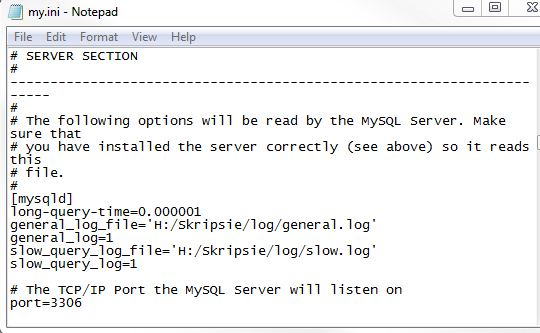
\includegraphics[scale = 0.65]{mysqlcom.jpg}	%http://www.mmogchart.com/Chart7.html how to ref?
%\caption{The configuration file of MySQL with logs enabled}
%\label{mysqlcom}
%\end{figure} %haal die dalk uit?

Enabling the general log in MySQL makes the server log each query that is made to the server from clients. This includes the type of query, the specific table it was made on and the time it was made. The response from the server is not logged at all however, which means that the general log does not provide any information on the amount of data that was sent back from the server or the time it took for each query to be sent. The general log is thus only useful to get an idea of how many queries are made to the database, and which queries occur the most.

Enabling the slow query log gives the user access to a little bit more information, but at a cost. It can slow down the response of the database under heavy load, but this was fortunately not a problem for the tests done on it. Another setback of the slow query log is that it only logs queries that take longer than a set amount of time. That value was set to 0.000001 seconds in the configuration file, which is its smallest possible value. The value is small enough that most queries made are logged, but some small queries happen faster than 0.000001 seconds and are then omitted from the logs. 

The following data is logged by the slow query log:

\begin{itemize}
	\item The time the query was made, rounded to the nearest second.
	\item The type of query made, the table it was made on and the user who made it.
	\item The amount of rows that were examined to make the query.
	\item The amount of rows that were sent back by the server as a result of the query.
	\item The time it took the server to find the right results of the query.
	\item The time it took the query to be completed.
\end{itemize}

With all of this data, a thorough analysis of the queries made to the database can be made and the average amount of queries made over time by players can be concluded with test data. The most frequent queries can also be determined as well as the time interval in between each query.

%Explain how MySQL works, how to access the tables contained in the database, how to make queries.
%Explain which logs are supported, how they work and how to enable them. Discuss the data that can be extracted from the logs and how they can be parsed by either your own program or using commercial software available for that purpose.


\section{MONyog} %prente maybe?

The usual text based command line interface of a MySQL server makes it difficult to use some of its features, and makes analysis of the databases it contains harder too. For this reason there exist many third-party applications that provide a more user-friendly GUI to use and analyse databases on a MySQL server. 

The data contained within the two logs that the MySQL server creates can be extracted by writing a parser program that takes a log file as input and parses the information it contains to calculate statistical data for the database. The amount of queries created over a certain amount of time, and the amount of times each query is made and so forth can be extracted in this way. There already exist third-party applications that provide this functionality however. MONyog is one of those applications,  and it was used to analyse the queries made to the ArcEmu MySQL databases.

MONyog sends status queries to the MySQL server every 5 minutes to get data on how the server performs throughout the day. This provides additional information about the database which can then be retrieved and analysed for the times that the WoW client was connected to the server.

MONyog also has the ability to parse both the general and the slow query log, to extract more information from them, which is displayed  in tabular format. All these analysis tools will be used to analyse how the database of the private WoW server responds to clients playing the game on it. Figure~\ref{monyog} shows the GUI provided by MONyog to analyse MySQL databases, with the current window showing the total size that the data of all the databases are taking up on the disk in megabytes. 


\begin{figure}[htbp]
\centering
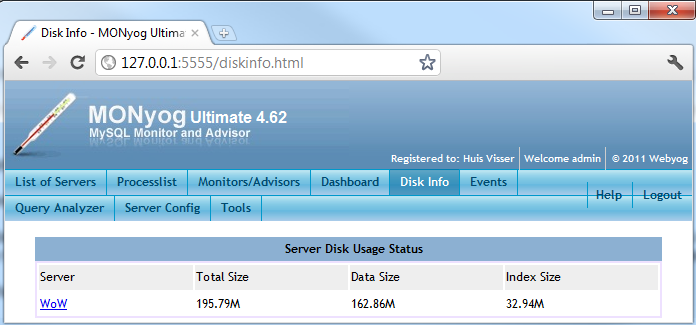
\includegraphics[scale = 0.65]{monyog.png}	
\caption{MONyog GUI showing the total size of the data contained in all the MySQL databases}
\label{monyog}
\end{figure}


%Briefly describe what MONyog is and how it works. Discuss how it enables users to analyse database data throughput and queries made to the database. Explain how the program was tested for accuracy and integrity of information, and show proof with images. Compare results found in logs to the output generated by monyog parser.


\section{Database Analysing Strategy}
\label{datastrategy}

With all the tools needed to analyse the databases and tables in place, a strategy is required on how to start characterising the data storage methods used by an MMORPG. A method is needed on how to determine when, why and how many queries are made to the database by the server. The nature and size of the queries are also of interest. 

From installing the databases it is known that the following data are contained in them:

\begin{itemize}
	\item The account information of all the users.
	\item The items, spells, skills, location and other data of every character that has been created.
	\item The NPCs, and quests they give and items they sell.
	\item All the mobs and where they are located and which loot the drop.
\end{itemize}


This data can give a general idea of what data needs to be saved and retrieved by the server, and what could be a trigger that causes the server to generate a query to the database. The account information would be needed to be compared to the data that users type in when they log into the server. It is probable that the server makes a query to the database to retrieve this information either in batch when the server is started, or every time a new user logs into the game.

When a user is logged in, the game goes to the character choosing or creating screen, where the user can either choose a character to log into the world with, or create a new character and then log into the world. For either of these options information about what skills and so forth the character will have is required, and it is probable that a query will be generated to the database every time a user creates a new character or chooses a character to play with.

When the user enters the world, the NPCs and the quests they give, as well as all the mobs, is already there. They continue to exist in the game world when the user logs out since other users might still be in the world. It is thus expected that all of this data is retrieved from the databases before any characters log in, as the server is started.

As the user is playing, the character will start quests, level up, gain skills and so forth. Many of these actions will change the properties of the user and this information needs to be saved in case the user logs out, so that it can be retrieved when the user decides to play again. It is therefore suspected that the following actions, among others, of any character will generate queries to the database:

\begin{itemize}
	\item Starting a quest.
	\item Completing a quest.
	\item Gaining any skill.
	\item Learning a new spell.
	\item Learning a new profession.
	\item Killing a mob.
	\item Picking up loot.
	\item Buying and selling items.
\end{itemize}

Whenever a player dies the character is turned into a ghost and teleported to the nearest graveyard. Information about where the nearest graveyard is or how the ghost must look would be needed, which suggests that another query would be made to the database by the server whenever a character dies. This could generate yet another query when the player finds its body and is reincarnated. 

After playing the game for a while, the user will log out of the world, and the server does not need to update other clients about the position of the user anymore. Any final data, such as the current position of the player and the current spells active and so forth also need to be saved. Queries would thus be generated whenever a character logs out of the game.


With a good idea of what actions in WoW will generate queries, a method is needed to test this expected behaviour. The general and slow query log will have a record of every query made, so a player could play the game and perform all of these actions and compare the logs with the time the actions were performed in the game. It would be better to isolate the data to get more precise results however. The following strategy will be followed in order to test whether the server behaves as expected:

The general and slow query logs will be activated and a user will log into the game. The logs will then be copied, saved and cleared before anything else is done in the game. After the logs are cleared, the user will choose a character to enter the game world, after which the logs will again be copied, saved and cleared. The user will then perform all the actions in the game that is suspected to generate queries, saving and clearing the logs after each action and labelling each log with the action it represents. Finally the user will log out and save the last logs. This should generate compelling data to analyse the behaviour of the server through every action that characters perform when playing the game.

After doing these tests and analysing them, a good picture can be formed on when and why the server stores and retrieves data. More data will still be needed to analyse whether this behaviour is consistent when a player plays the game for a long time, and even more importantly, when more than one player is playing at the same time. To determine this, more tests are needed.


\subsection{Further Tests} %better name?
\label{further}

All the data that will be collected up till now will be very fractioned and only relevant to one specific action. To gain information about the behaviour of the server in general, the logs will once again be enabled and a user will log in and play the game normally for three hours. It is of interest to determine how much queries are generated by a player in a typical gaming session, what the most frequent queries are, and the inter-arrival time of the queries in general. 

Of further interest is how the server responds when more than one player is logged in simultaneously and playing the game. To simulate more players on the server, a program called a bot (short for robot) is used. This program is able to control a WoW character and play the game to a certain extent. It follows a path that has been set out for it specifically, and attacks, kills and loots mobs on that pathway. Quests need to be started and completed manually however, and the behaviour of the character is not the same as that of a human player, but its the closest that can be simulated.

Up to four characters can be logged onto the same server by using this software. These test will be done and further discussed in chapter~\ref{results}, where the results of the tests will also be analysed.

%Now that it is known which actions in the game cause which queries, tests need to be done to determine how much queries are generated by a player playing the game normally for a gaming session. It is also of interest if the queries multiply with the amount of players when more players are playing the game. The most frequent queries and their inter-arrival time is also of interest to be able to create a model of normal database behaviour.
%
%To simulate more players on the server, a program called a bot (short for robot) is used. This program is able to control a WoW character and play the game to a certain extent. It follows a path that has been set out for it specifically, and attacks, kills and loots mobs on that pathway. Quests need to be started and completed manually however, and the behaviour of the character is not the same as that of a human player, but its the closest that can be simulated.
%
%Up to four characters can be logged onto the same server by using this software. These test will be done and further discussed in chapter \ref{results}, where the results will be of the tests will also be analysed.

%With the tools needed to analyse the databases and tables in place, more information is needed on which actions of the character causes which queries to be generated. To gather this information the general and slow query logs are needed. Before starting with this exercise a list of actions done by the character that is expected to change some game-state which would generate a query of some sort is made. This includes things such as killing mobs, taking loot, logging in, doing and finishing quests, gaining skills and leveling up, to  name a few. 
%
%At first the logs were cleared completely. After that a certain action was performed in the game and the logs were copied and saved after performing the action. The logs were then cleared once again before the next action was performed and so forth. With this method, several actions and their associated queries were saved for further analysis. 
%
%What was surprising was that the following behaviour from the database was found: most of the actions performed by the character did not generate immediate queries. The expected queries did however happen  a few seconds or even minutes after the action was performed. This suggests that the server saves all actions that will generate queries in variables at first. A queue of queries is then created that is executed either when the queue gets too full or after a certain interval. There are however certain actions that always generated immediate queries. This could mean that those queries are either big enough for the queue of queries to be considered full enough to be executed, or they are simply of higher priority and thus handled immediately. When any query is executed however, the queue is emptied and all the queries that did not take place immediately is executed along with the others.
%
%This behaviour from the server makes sense upon reflecting on it, since it would concentrate queries made to the database when a small amount of queries need to be made. Extensive testing was done to test this expected server behaviour, but after generating as much queries as possible with five clients logged in simultaneously, the queries still only happened after a counter of sorts triggered the queries to be made. This suggests that the server has a timer that generates an interrupt of sorts after a set amount of time has passed. This interrupt then causes the server to make all the queries that are needed to the database. This is the equivalent of saving all the changes that have happened in the meantime.
%
%It is sensible for the server to behave in this way, because the server has a lot of other things that it is responsible for, such as generating all the actions of the mobs and sending location information to all the clients and so forth. If every action that caused a change in game state generated an immediate query then the server would constantly be busy sending information to the database, causing lag in its normal and more important function of communicating with the client. This behaviour would become worse when more clients connect to the server, and the game would soon become unplayable. 
%
%The following pattern was discovered by analysing hundreds of queries made to the database to ensure its legitimacy: there are two counters that generate queries constantly looping on the server side. The one counter generates a query to check if any of the players has sent mail to any of the other players every three minutes. This is the shorter of the two counters, which is understandable because other players could be waiting for the mail to be sent, which makes it a higher priority query.
%
%The other counter generates a ``START TRANSACTION'' query every five minutes. This query starts a sequence of queries that save all the changes to all the characters that have happened in the past five minutes. This includes all new skills and spells learned, gold collected, quests accepted and completed and so forth. 
%
%Table \ref{queries} lists all the actions that were found to generate queries immediately, as well as the amount of queries that they generate. The queries generated by starting the ArcEmu server are also listed. Starting ArcEmu generates the largest amount of queries by far, but this should only happen once per week at a maximum, when servers are restarted for maintenance purposes.
%
%
%\begin{table}[htbp]
%  \centering
%  \caption{List of actions in WoW that generate immediate queries}
%    \begin{tabular}{lrlr}
%    \addlinespace
%    \toprule
%    \textbf{Action in game} & \textbf{} & \textbf{Queries} & \textbf{Total time to execute} \\
%    \midrule
%    Starting ArcEmu &       & 1845 queries & 27.199 sec \\
%    \midrule
%    Logging in &       & 3 queries & 1.047 sec \\
%    \midrule
%    Creating a character &       & 18 queries & 0.765 sec \\
%    \midrule
%    Entering World &       & 23 queries & 0.597 sec \\
%    \midrule
%    Selling Items &       & 1  query & 0.056 sec \\
%          &       & per item &  \\
%    \midrule
%    Dying &       & 2 queries & 0.059 sec \\
%    \midrule
%    Resurrecting &       & 1  query & 0.049 sec \\
%    \midrule
%    Logging Out &       & 76 queries & 0.078 sec \\
%    \bottomrule
%    \end{tabular}%
%  \label{queries}%
%\end{table}%
%
%
%All of these actions in WoW are of high priority, which is why the server deems them important enough to break its usual cycle of only saving changes to the database every few minutes. Most of these actions only happen once per gaming session however, so they should not have a large effect on the performance of the server.
%
%The actions in the game that happen most frequently, like gaining skill points, levelling up and starting and completing quests are all processed at the same time, and only add one query per action to the list. Attributes like which spells a character knows and which items are in their backpacks are all both deleted and inserted into the database every five minutes with the START TRANSACTION query that happens. This will happen even if the character does nothing in that time. Analysing several logs revealed that the START TRANSACTION query generates approximately 65 queries for every player every 5 minutes when the player does nothing.

%Discuss how the game was played for hours to generate queries, explain what was done in game and which corresponding queries were created for each action. Mention resulting queries from playing for 3 hours and how database reacted etc.


%\section{Database Tests} %better name?
%Now that it is known which actions in the game cause which queries, tests need to be done to determine how much queries are generated by a player playing the game normally for a gaming session. It is also of interest if the queries multiply with the amount of players when more players are playing the game. The most frequent queries and their inter-arrival time is also of interest to be able to create a model of normal database behaviour.
%
%To simulate more players on the server, a program called a bot (short for robot) is used. This program is able to control a WoW character and play the game to a certain extent. It follows a path that has been set out for it specifically, and attacks, kills and loots mobs on that pathway. Quests need to be started and completed manually however, and the behaviour of the character is not the same as that of a human player, but its the closest that can be simulated.
%
%Up to four characters can be logged onto the same server by using this software. These test will be done and further discussed in chapter \ref{results}, where the results will be of the tests will also be analysed. %This was done and the reaction of the database was compared to the data captured with only one human player playing the game. These results are analysed and compared in chapter \ref{results}.

%Not sure if this belongs here? Mention resulting queries from playing for 3 hours and how database reacted etc. and how bots were added. Explain results expected from adding bots, show results from adding them and explain differences.
%Will have to be careful to not go into too much detail since this needs to be discussed in a separate chapter in more detail. Perhaps only mention that the tests were done here and leave the results for later?




%\begin{table}[htbp]
%  \centering
%  \caption{List of actions in WoW that generate immediate queries}
%    \begin{tabular}{lrlr}
%    \addlinespace
%    \toprule
%    \textbf{Action in game} & \textbf{} & \textbf{Queries} & \textbf{Total time to execute} \\
%    \midrule
%    Starting ArcEmu &       & 2 UPDATE queries & 27.199 sec \\
%          &       & 2 INSERT queries &  \\
%          &       & 3 DELETE queries &  \\
%          &       & 13 Connect queries &  \\
%          &       & 1825 SELECT queries &  \\
%    \midrule
%    Logging in &       & 1 UPDATE query & 1.047 sec \\
%          &       & 2 SELECT queries &  \\
%    \midrule
%    Creating a character &       & 5 SELECT queries & 0.765 sec \\
%          &       & 13 DELETE queries &  \\
%    \midrule
%    Entering World &       & 1 UPDATE query & 0.597 sec \\
%          &       & 1 DELETE query &  \\
%          &       & 2 INSERT queries &  \\
%          &       & 19 SELECT queries &  \\
%    \midrule
%    Selling Items &       & 1 DELETE query & 0.056 sec \\
%          &       & per item &  \\
%    \midrule
%    Dying &       & 1 DELETE query & 0.059 sec \\
%          &       & 1 INSERT query &  \\
%    \midrule
%    Resurrecting &       & 1 DELETE query & 0.049 sec \\
%    \midrule
%    Logging Out &       & 1 COMMIT query & 0.078 sec \\
%          &       & 4 SELECT queries &  \\
%          &       & 20 DELETE queries &  \\
%          &       & 51 INSERT queries &  \\
%    \bottomrule
%    \end{tabular}%
%  \label{queries}%
%\end{table}%